\chapter{Prova de Conceito DevSecOps com Infraestrutura Local Baseada em Contêineres}
\label{apendice:poc-devsecops}

Este apêndice apresenta a Prova de Conceito (PoC) desenvolvida como parte desta monografia, cujo objetivo é validar, de forma prática, o modelo proposto de esteira DevSecOps aliado ao conceito de Infraestrutura como Código (IaC).

Diferentemente de uma implementação tradicional em nuvem pública, a PoC foi projetada para operar integralmente em ambiente local, utilizando contêineres Docker como abstração dos principais serviços de uma arquitetura baseada na Amazon Web Services (AWS). Essa abordagem permite reprodutibilidade, baixo custo operacional e maior controle sobre o ambiente de experimentação.

\section{Objetivo da Prova de Conceito}

A Prova de Conceito tem como principal objetivo demonstrar a viabilidade técnica da aplicação integrada de práticas DevSecOps em conjunto com IaC, simulando um fluxo completo de provisionamento, validação, segurança e execução de aplicações.

Especificamente, busca-se:

\begin{itemize}
\item Validar a automação de infraestrutura utilizando Terraform;
\item Demonstrar a execução de uma pipeline DevSecOps com análise de segurança integrada;
\item Simular serviços típicos de nuvem (rede, banco de dados e aplicação) em ambiente local;
\item Garantir reprodutibilidade por meio de scripts automatizados;
\item Evidenciar a aplicação de boas práticas de segurança em contêineres e código IaC.
\end{itemize}

\section{Visão Geral da Arquitetura}

A arquitetura da PoC foi concebida para refletir, de maneira simplificada, uma infraestrutura baseada em serviços AWS, utilizando contêineres Docker como substitutos funcionais.

A correspondência entre os componentes simulados e seus equivalentes na nuvem é apresentada a seguir:

\begin{itemize}
  \item \textbf{VPC} -> Rede Docker dedicada (\texttt{docker\_network});
  \item \textbf{Amazon RDS} -> Contêiner PostgreSQL com volume persistente;
  \item \textbf{Amazon EKS / ECS} -> Múltiplas réplicas de aplicações FastAPI;
  \item \textbf{Elastic Load Balancer} -> Servidor NGINX atuando como proxy reverso;
  \item \textbf{Secrets Manager / Parameter Store} -> Variáveis de ambiente (.env).
\end{itemize}

O fluxo de comunicação ocorre da seguinte forma:

\begin{center}
Cliente $\rightarrow$ NGINX (balanceador) $\rightarrow$ APIs FastAPI $\rightarrow$ PostgreSQL
\end{center}

Todos os contêineres são conectados a uma rede Docker única, simulando o isolamento de uma VPC.

\begin{figure}[ht]
    \caption{ Diagrama de arquitetura da esteira DevSecOps integrada, detalhando o fluxo de trabalho desde o código-fonte até o ambiente de nuvem, destacando os portões de validação (SAST, SCA e Secrets Detection) que atuam como barreiras de conformidade. }
    \label{fig:cvss}
    \centering
    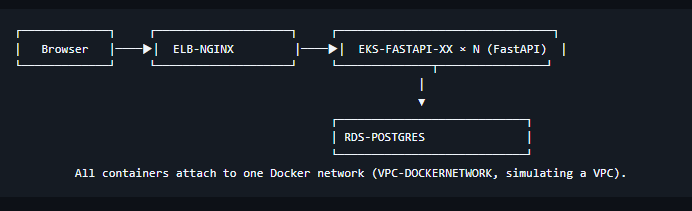
\includegraphics[width=0.8\textwidth]{Arquivos/figuras/Figura_Arquitetura_PoC_Containers.png}
    \fonte{Elaborado pelo autor}
\end{figure}

\section{Ferramentas e Tecnologias Utilizadas}

A PoC utiliza um conjunto de ferramentas amplamente adotadas no contexto DevSecOps:

\begin{itemize}
\item \textbf{Terraform}: provisionamento declarativo da infraestrutura local;
\item \textbf{Docker}: execução e isolamento dos serviços simulados;
\item \textbf{Checkov}: análise estática de segurança para código IaC e Dockerfiles;
\item \textbf{GitHub Actions}: automação da pipeline CI/CD;
\item \textbf{NGINX}: balanceamento de carga entre serviços;
\item \textbf{FastAPI}: implementação da camada de aplicação;
\item \textbf{PostgreSQL}: persistência de dados.
\end{itemize}

\section{Execução Automatizada do Ambiente}

Um dos diferenciais da PoC é a possibilidade de provisionamento completo do ambiente por meio de um único comando:

\begin{verbatim}
./dev-up.sh
\end{verbatim}

Esse script realiza automaticamente:

\begin{itemize}
\item Verificação de dependências (Docker e Terraform);
\item Criação do arquivo de configuração (.env);
\item Execução da análise de segurança com Checkov;
\item Inicialização e aplicação do Terraform;
\item Provisionamento dos contêineres;
\item Exibição de informações para inspeção do ambiente.
\end{itemize}

Também é possível executar o teardown completo com:

\begin{verbatim}
./dev-down.sh
\end{verbatim}

\section{Estrutura do Projeto}

A organização do repositório segue uma abordagem modular e alinhada às boas práticas de engenharia de software:

\begin{verbatim}
|-- terraform/
|   |-- network/
|   |-- database/
|   |-- backend/
|   |-- frontend/
|   \-- main.tf
|
|-- app/
|   |-- backend/
|   \-- frontend/
|
|-- scripts/
|   |-- dev-up.sh
|   \-- terraform-docker.sh
|
|-- .github/workflows/
|   \-- pipeline.yml
|
|-- docker-compose.yml
|-- Makefile
\-- README.md
\end{verbatim}

Essa estrutura permite separação clara entre infraestrutura, aplicação e automação.

\section{Pipeline DevSecOps}

A pipeline CI/CD definida no projeto automatiza as principais etapas de validação e segurança:

\begin{enumerate}
\item Validação de formatação do Terraform (\textit{terraform fmt});
\item Inicialização e validação da infraestrutura (\textit{init e validate});
\item Análise de segurança com Checkov:
\begin{itemize}
\item Código Terraform (IaC);
\item Dockerfiles (boas práticas de containers);
\end{itemize}
\item Geração do plano de execução (\textit{terraform plan}).
\end{enumerate}

A pipeline é configurada para falhar automaticamente caso vulnerabilidades críticas sejam identificadas.

\section{Segurança e Boas Práticas}

Durante o desenvolvimento da PoC, foram identificadas e corrigidas vulnerabilidades comuns, tais como:

\begin{itemize}
\item Ausência de \textit{HEALTHCHECK} em contêineres;
\item Execução de processos como usuário root;
\item Uso indevido de contêineres privilegiados;
\end{itemize}

As correções implementadas incluem:

\begin{itemize}
\item Definição explícita de usuários não privilegiados;
\item Configuração de \textit{HEALTHCHECK} nos serviços;
\item Uso de imagens seguras (ex: nginx não privilegiado);
\item Desativação de privilégios elevados nos contêineres.
\end{itemize}

Essas práticas reforçam a integração entre segurança e desenvolvimento, princípio central do DevSecOps.

\section{Execução e Validação}

Após a execução da PoC, o ambiente pode ser acessado via navegador:

\begin{verbatim}
http://localhost:3000
\end{verbatim}

Também é possível validar o funcionamento da API:

\begin{verbatim}
curl http://localhost:3000/api/status
\end{verbatim}

E inspecionar os contêineres:

\begin{verbatim}
docker ps
\end{verbatim}

\section{Evidências e Reprodutibilidade}

A PoC foi projetada para ser totalmente reprodutível, permitindo que qualquer usuário com Docker instalado consiga executar o ambiente localmente.

O repositório contém:

\begin{itemize}
\item Código-fonte da infraestrutura e aplicação;
\item Scripts de automação;
\item Pipeline CI/CD configurada;
\item Documentação detalhada de uso e experimentação.
\end{itemize}

\begin{quote}
\textbf{Repositório:} \url{https://github.com/miguel-henrique/poc-devsecops/}
\end{quote}


\subsection{Saída da Pipeline}

A execução da pipeline DevSecOps gera saídas que evidenciam cada etapa do processo de validação, segurança e provisionamento da infraestrutura. Os resultados apresentados a seguir demonstram a aplicação prática das ferramentas integradas, permitindo observar desde a análise de segurança até a criação dos recursos e inicialização dos serviços.

A seguir são apresentados trechos da saída da pipeline DevSecOps executada durante a Prova de Conceito.

\begin{figure}[ht]
    \caption{ Resultado da análise estática de segurança realizada pelo Checkov nos Dockerfiles do projeto. A execução apresenta 72 verificações aprovadas, nenhuma falha crítica e algumas verificações ignoradas, demonstrando conformidade com boas práticas de segurança, como a não utilização do usuário root, restrição de portas sensíveis e uso adequado de instruções no Dockerfile. }
    \label{fig:cvss}
    \centering
    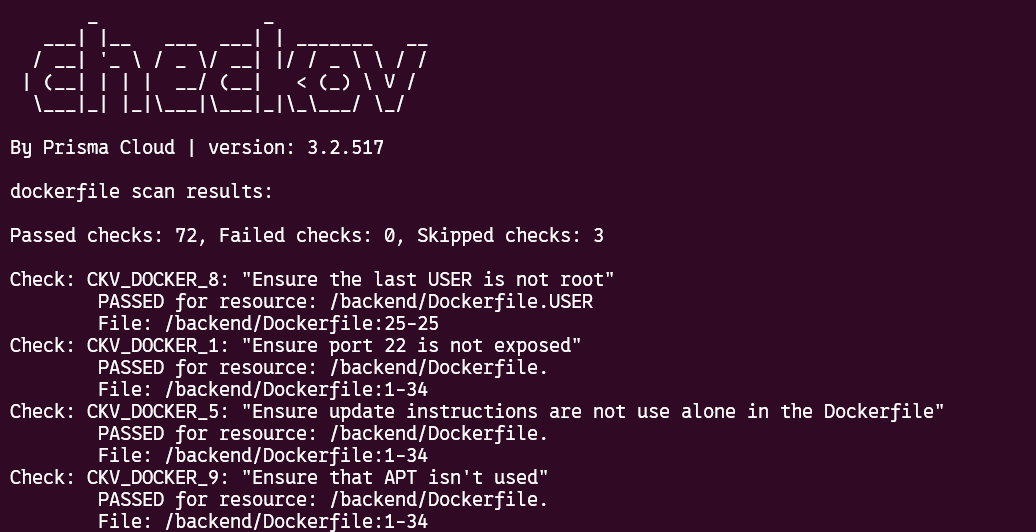
\includegraphics[width=0.8\textwidth]{Arquivos/figuras/Figura_Output_PoC_Checkov.png}
    \fonte{Elaborado pelo autor}
\end{figure}

\begin{figure}[ht]
    \caption{ Saída do comando \textit{terraform plan}, evidenciando a detecção de mudanças na infraestrutura e a definição dos recursos a serem criados. Observa-se a adição de componentes como configurações de rede (subnet) e metadados (labels), totalizando dez novos recursos a serem provisionados, sem alterações ou destruições, garantindo previsibilidade e controle sobre o estado da infraestrutura. }
    \label{fig:cvss}
    \centering
    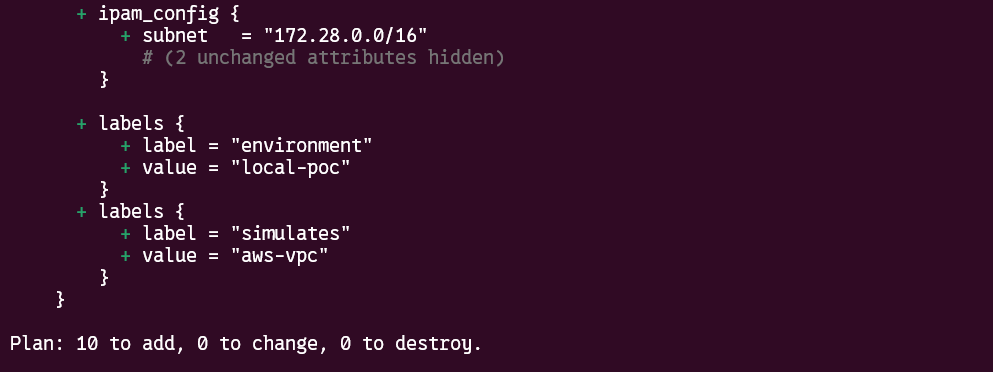
\includegraphics[width=0.8\textwidth]{Arquivos/figuras/Figura_Output_PoC_Terraform_Plan.png}
    \fonte{Elaborado pelo autor}
\end{figure}

\begin{figure}[ht]
    \caption{ Listagem dos contêineres em execução após o provisionamento do ambiente, representando a simulação da arquitetura em nuvem. Observa-se o balanceador NGINX exposto na porta 3000, múltiplas instâncias da aplicação FastAPI e o banco de dados PostgreSQL, todos em processo de inicialização (\textit{health: starting}), evidenciando o funcionamento integrado da infraestrutura local baseada em contêineres. }
    \label{fig:cvss}
    \centering
    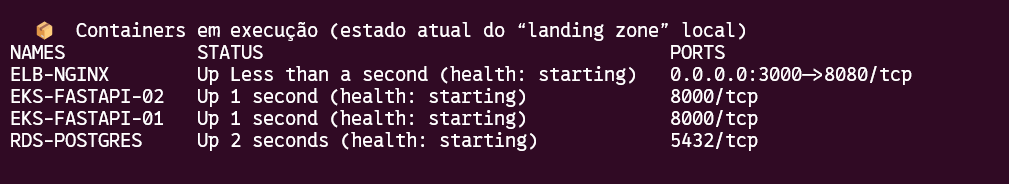
\includegraphics[width=0.8\textwidth]{Arquivos/figuras/Figura_Output_PoC_Container.png}
    \fonte{Elaborado pelo autor}
\end{figure}


\section{Considerações Finais}

A Prova de Conceito demonstrou que é possível implementar uma esteira DevSecOps completa sem dependência direta de provedores de nuvem, utilizando abstrações locais baseadas em contêineres.

Os resultados evidenciam que:

\begin{itemize}
\item A integração entre IaC, segurança e automação é viável e eficiente;
\item Ferramentas como Terraform e Checkov podem ser aplicadas mesmo fora de ambientes cloud;
\item A abordagem local facilita testes, aprendizado e validação de arquiteturas complexas;
\item O modelo proposto é facilmente adaptável para ambientes reais em nuvem.
\end{itemize}

Dessa forma, a PoC serve como uma base sólida para evolução futura e aplicação em cenários corporativos reais, mantendo os princípios fundamentais de DevSecOps.
